\section*{Introduction}
\phantomsection
A control structure is a block of programming that analyzes variables and chooses a direction in which to go based on given parameters. The term \textit{flow control} details the direction the program takes (which way program control "flows"). Hence it is the basic decision-making process in computing; flow control determines how a computer will respond when given certain conditions and parameters.\newline

Those initial conditions and parameters are called preconditions. Preconditions are the state of variables before entering a control structure. Based on those preconditions, the computer runs an algorithm (the control structure) to determine what to do. The result is called a postcondition. Postconditions are the state of variables after the algorithm is run. \newline

According to the structure theorem, any computer program can be written using the basic control structures shown in Figure 1. They can be combined in any way necessary to deal with a given problem.

\begin{figure}[ht!]
    \centering
	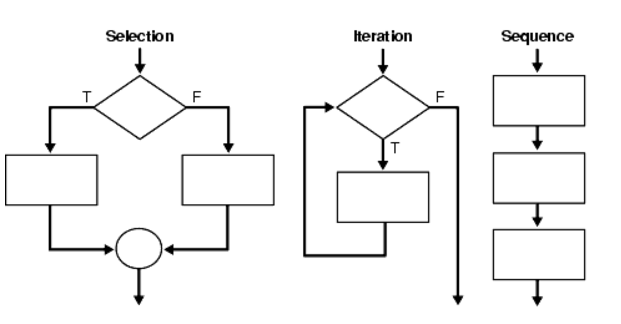
\includegraphics{images/Figure1.png}
    \caption{Control Structures}
    \label{fig1}
\end{figure}
The \textit{selection} structure tests a condition, then executes one sequence of statements instead of another, depending on whether the condition is true or false. A condition is any variable or expression that returns a Boolean value (TRUE or FALSE). The \textit{iteration} structure executes a sequence of statements repeatedly as long as a condition holds true. The \textit{sequence} structure simply executes a sequence of statements in the order in which they occur.


\clearpage